\documentclass[UTF8,a4paper,zihao=-4]{ctexart}

\usepackage{geometry}
\geometry{left=2.5cm,right=2.5cm,top=2.6cm,bottom=2.6cm}
\usepackage{amsmath,amssymb,bm}
\usepackage{graphicx}
\usepackage{booktabs}
\usepackage{caption}
\usepackage{subcaption}
\usepackage{float}
\usepackage{siunitx}
\usepackage{hyperref}
\usepackage{cleveref}
\usepackage{enumitem}
\usepackage{array}
\usepackage{xcolor}

\hypersetup{
  colorlinks=true,
  linkcolor=black,
  citecolor=black,
  urlcolor=black
}

\captionsetup{font=small,labelfont=bf}
\setlength{\parindent}{2em}
\setlength{\parskip}{0pt}
\linespread{1.18}
\emergencystretch=2em
\graphicspath{{../assets/}{../assets/q3_visualization/}{../assets/q3_fem/}{../assets/q3_comparison/}}
\crefname{figure}{图}{图}
\crefname{table}{表}{表}
\crefname{equation}{式}{式}
\crefname{subfigure}{图}{图}

\ctexset{
  section = {
    format = \zihao{4}\bfseries,
    name = {,、},
    number = \chinese{section}
  },
  subsection = {
    format = \zihao{-4}\bfseries
  }
}

\title{\heiti 带集中质量与局部弹簧支承 Euler--Bernoulli 梁自由振动的解析解与有限元验证}
\author{
  王子传\quad 吕天翔\quad 方思哲\\
  \small 天津大学机械工程学院
}
\date{}

\begin{document}

\maketitle

\begin{abstract}
针对一类含内点外部铰支、集中质量和局部竖向弹簧支承的均质等截面 Euler--Bernoulli 梁，研究其横向自由振动特性。首先基于分离变量法建立梁段振动方程，并通过传递矩阵法处理铰支反力、集中质量惯性和弹簧弹性力引起的状态跳跃，得到系统频率方程、振型函数及初速度作用下的模态响应表达式。其次，采用二节点 Hermite 梁单元建立有限元模型，将集中质量与弹簧分别并入整体质量矩阵和刚度矩阵，并通过位移自由度消元施加铰支约束。最后，在无量纲参数 $\alpha=m/(\rho Sl)=0.5$、$\kappa=kl^3/(EJ)=20$ 下对解析解与有限元结果进行对比。结果表明，有限元前若干阶固有频率与解析解吻合良好，前四阶振型节点相对误差约为 $10^{-9}$ 至 $10^{-8}$ 量级，动力响应差异主要来源于高阶模态截断和空间离散误差。研究结果可为含局部附件与局部弹性约束梁结构的动力学建模与数值验证提供参考。
\end{abstract}

\noindent\textbf{关键词：}Euler--Bernoulli 梁；自由振动；传递矩阵法；集中质量；弹簧支承；有限元法

\section{引言}

梁结构是机械、土木、航空航天和交通装备中最常见的承载构件之一。对于细长梁结构，其横向振动特性常可采用 Euler--Bernoulli 梁理论描述。实际工程中，梁上常存在局部支承、附加质量、传感器、执行器或弹性连接等离散构件，这些局部因素会改变结构的固有频率、振型分布及瞬态响应特征。因此，建立能够同时处理连续梁段和离散构件的动力学模型具有重要意义。

对于均匀梁的振动问题，经典解析方法包括分离变量法、模态叠加法和传递矩阵法等。传递矩阵法能够以状态向量形式表达梁段内解，并通过跳跃矩阵处理集中质量、弹簧和集中力等局部作用，适合求解具有分段连续特征的梁结构。另一方面，有限元法具有良好的通用性和可扩展性，可通过 Hermite 梁单元对 Euler--Bernoulli 梁进行空间离散，并方便地引入集中质量、弹簧和支承约束。将解析解与有限元结果进行对比，可同时验证理论推导和数值实现的正确性。

本文研究如\cref{fig:model} 所示的梁结构。梁总长为 $4l$，在 $B$ 点通过外部铰支座与地面连接，在 $C$ 点附加集中质量 $m$，在 $D$ 点通过竖向线性弹簧与地面连接。本文首先推导该结构横向自由振动的解析解，然后建立有限元模型，最后从固有频率、振型函数和动力响应三个方面进行对比分析。

\begin{figure}[H]
  \centering
  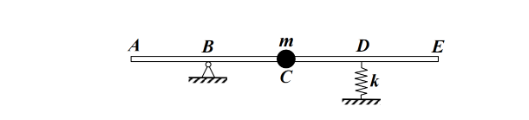
\includegraphics[width=0.62\linewidth]{image-20260616001638017.png}
  \caption{带集中质量与局部弹簧支承梁结构示意图}
  \label{fig:model}
\end{figure}

\section{结构模型与解析解}

\subsection{控制方程与无量纲参数}

取梁左端 $A$ 为坐标原点，沿梁轴线向右建立坐标 $x$，则
\begin{equation}
A:x=0,\quad B:x=l,\quad C:x=2l,\quad D:x=3l,\quad E:x=4l .
\end{equation}
梁的横向位移记为 $w(x,t)$。设梁线密度为
\begin{equation}
\mu=\rho S ,
\end{equation}
则除局部支承和集中质量位置外，Euler--Bernoulli 梁横向自由振动控制方程为
\begin{equation}
EJ\frac{\partial^4 w}{\partial x^4}+\mu\frac{\partial^2 w}{\partial t^2}=0 .
\label{eq:governing}
\end{equation}

令
\begin{equation}
w(x,t)=\phi(x)q(t),
\end{equation}
代入\cref{eq:governing} 可得
\begin{equation}
\phi^{(4)}(x)-\lambda^4\phi(x)=0,\qquad
\omega=\lambda^2\sqrt{\frac{EJ}{\rho S}} .
\end{equation}
进一步引入无量纲坐标与频率参数
\begin{equation}
\xi=\frac{x}{l},\qquad \beta=\lambda l ,
\end{equation}
并记 $Y(\xi)=\phi(x)$，则空间方程化为
\begin{equation}
Y''''-\beta^4Y=0,
\label{eq:dimensionless_beam}
\end{equation}
固有圆频率为
\begin{equation}
\omega_n=\frac{\beta_n^2}{l^2}\sqrt{\frac{EJ}{\rho S}} .
\label{eq:omega_beta}
\end{equation}

\subsection{边界条件与局部连接条件}

梁两端 $A$ 与 $E$ 均为自由端，故满足
\begin{equation}
Y''(0)=Y'''(0)=0,\qquad
Y''(4)=Y'''(4)=0 .
\end{equation}

本文将 $B$ 点视为连续梁上的外部简单支承点，而非梁内铰。因此 $B$ 点满足位移约束
\begin{equation}
Y(1)=0 ,
\end{equation}
同时位移、转角和弯矩连续，剪力可因支座反力发生跳跃。

$C$ 点集中质量只提供横向惯性。对集中质量位置作局部平衡，并代入简谐振动形式，可得
\begin{equation}
Y'''(2^+)-Y'''(2^-)=\alpha\beta^4Y(2),
\qquad
\alpha=\frac{m}{\rho Sl}.
\label{eq:mass_jump}
\end{equation}
$D$ 点竖向线性弹簧引起的状态跳跃为
\begin{equation}
Y'''(3^+)-Y'''(3^-)=-\kappa Y(3),
\qquad
\kappa=\frac{kl^3}{EJ}.
\label{eq:spring_jump}
\end{equation}

\subsection{传递矩阵形式}

定义状态向量
\begin{equation}
\bm z(\xi)=
\begin{bmatrix}
Y(\xi)&Y'(\xi)&Y''(\xi)&Y'''(\xi)
\end{bmatrix}^{\mathrm T}.
\end{equation}
由\cref{eq:dimensionless_beam} 可得梁段传递关系
\begin{equation}
\bm z(\xi+s)=\bm P(s)\bm z(\xi),
\end{equation}
其中 $\bm P(s)$ 为 Euler--Bernoulli 梁段传递矩阵。记
\begin{equation}
C_h=\cosh \beta s,\quad S_h=\sinh \beta s,\quad C=\cos \beta s,\quad S=\sin \beta s,
\end{equation}
则
\begin{equation}
\bm P(s)=
\begin{bmatrix}
\frac{C_h+C}{2} & \frac{S_h+S}{2\beta} & \frac{C_h-C}{2\beta^2} & \frac{S_h-S}{2\beta^3}\\
\frac{\beta(S_h-S)}{2} & \frac{C_h+C}{2} & \frac{S_h+S}{2\beta} & \frac{C_h-C}{2\beta^2}\\
\frac{\beta^2(C_h-C)}{2} & \frac{\beta(S_h-S)}{2} & \frac{C_h+C}{2} & \frac{S_h+S}{2\beta}\\
\frac{\beta^3(S_h+S)}{2} & \frac{\beta^2(C_h-C)}{2} & \frac{\beta(S_h-S)}{2} & \frac{C_h+C}{2}
\end{bmatrix}.
\label{eq:P}
\end{equation}

集中质量和弹簧对应的跳跃矩阵分别为
\begin{equation}
\bm J_m=
\begin{bmatrix}
1&0&0&0\\
0&1&0&0\\
0&0&1&0\\
\alpha\beta^4&0&0&1
\end{bmatrix},\qquad
\bm J_k=
\begin{bmatrix}
1&0&0&0\\
0&1&0&0\\
0&0&1&0\\
-\kappa&0&0&1
\end{bmatrix}.
\end{equation}

由于左端自由，可令
\begin{equation}
\bm z(0)=
\begin{bmatrix}
a&b&0&0
\end{bmatrix}^{\mathrm T}.
\end{equation}
设 $B$ 点支座引起的无量纲剪力跳跃为 $R$，则
\begin{equation}
\bm z(1^+)=\bm P(1)\bm z(0)+R\bm e_4 ,
\end{equation}
其中 $\bm e_4=[0,0,0,1]^{\mathrm T}$。定义
\begin{equation}
\bm T(\beta)=\bm P(1)\bm J_k\bm P(1)\bm J_m\bm P(1),
\end{equation}
则右端状态为
\begin{equation}
\bm z(4)=\bm T(\beta)\left[\bm P(1)
\begin{bmatrix}
a\\b\\0\\0
\end{bmatrix}
+R\bm e_4\right].
\end{equation}
结合 $B$ 点位移约束和 $E$ 端自由边界条件，可得齐次线性方程
\begin{equation}
\bm A(\beta)\bm c=\bm 0,\qquad
\bm c=
\begin{bmatrix}
a&b&R
\end{bmatrix}^{\mathrm T}.
\end{equation}
非平凡解存在的条件为
\begin{equation}
\det \bm A(\beta)=0 .
\label{eq:char_eq}
\end{equation}
求解\cref{eq:char_eq} 可得频率参数 $\beta_n$，再由\cref{eq:omega_beta} 得到固有频率。

\subsection{模态响应}

对每一阶特征根 $\beta_n$，由 $\bm A(\beta_n)\bm c_n=\bm 0$ 可求得对应振型 $\phi_n(x)$。考虑初始位移为零，且初始广义动量由 $C$ 点集中质量速度 $v_0$ 提供，则梁的自由响应为
\begin{equation}
w(x,t)=
\sum_{n=1}^{\infty}
\phi_n(x)
\frac{m v_0\phi_n(2l)}
{M_n\omega_n}
\sin\omega_n t ,
\label{eq:response}
\end{equation}
其中模态质量为
\begin{equation}
M_n=
\int_0^{4l}\rho S\phi_n^2(x)\,\mathrm dx+
m\phi_n^2(2l).
\end{equation}

\section{有限元模型}

\subsection{梁单元矩阵}

有限元计算采用二节点 Euler--Bernoulli Hermite 梁单元，每个节点包含横向位移 $w$ 和转角 $\theta$ 两个自由度。设单元长度为 $h$，则单元刚度矩阵为
\begin{equation}
\bm k_e=\frac{EJ}{h^3}
\begin{bmatrix}
12&6h&-12&6h\\
6h&4h^2&-6h&2h^2\\
-12&-6h&12&-6h\\
6h&2h^2&-6h&4h^2
\end{bmatrix}.
\end{equation}
采用一致质量矩阵
\begin{equation}
\bm m_e=\frac{\rho S h}{420}
\begin{bmatrix}
156&22h&54&-13h\\
22h&4h^2&13h&-3h^2\\
54&13h&156&-22h\\
-13h&-3h^2&-22h&4h^2
\end{bmatrix}.
\end{equation}

\subsection{局部构件与边界约束}

整体矩阵组装完成后，将 $C$ 点集中质量加入对应节点平动质量自由度，将 $D$ 点弹簧刚度加入对应节点平动刚度自由度。$B$ 点铰支座通过消元法施加 $w_B=0$，并保留其转角自由度。由此得到广义特征值问题
\begin{equation}
\bm K\bm \Phi_n=\omega_n^2\bm M\bm \Phi_n .
\label{eq:fem_eigen}
\end{equation}
在无量纲计算中取梁长为 $4$，分布质量和弯曲刚度均归一化。本文采用 $80$ 个梁单元，节点数为 $81$，响应计算中叠加前 $24$ 阶模态。

\section{数值结果与对比}

\subsection{计算参数}

本文采用无量纲参数
\begin{equation}
\alpha=0.5,\qquad \kappa=20 .
\end{equation}
无量纲频率定义为
\begin{equation}
\bar\omega_n=\omega_n l^2\sqrt{\frac{\rho S}{EJ}}=\beta_n^2 .
\end{equation}
有限元程序采用 Fortran 编写，结果导出为 CSV 文件；后处理和绘图采用 Python 与 SciencePlots 完成。

\subsection{解析解可视化}

在进行有限元验证前，首先对解析传递矩阵解进行可视化。\cref{fig:analytical_roots} 给出了特征方程 $\det\bm A(\beta)=0$ 的扫描结果及前若干阶根的位置。可以看到，特征函数在正根处发生过零，所得根值进一步代入\cref{eq:omega_beta} 即可得到对应固有频率。

\begin{figure}[H]
  \centering
  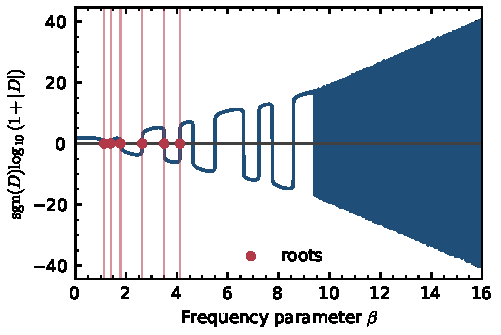
\includegraphics[width=0.62\linewidth]{q3_characteristic_roots.pdf}
  \caption{解析特征方程及特征根分布}
  \label{fig:analytical_roots}
\end{figure}

\cref{fig:analytical_modes_response} 给出了由解析解得到的前四阶归一化振型以及全梁时空响应。振型在 $B$ 点满足位移约束，在 $C$、$D$ 点保持位移连续，同时通过状态跳跃反映集中质量和弹簧支承的局部作用。时空响应图反映了初速度作用后全梁横向位移随时间和空间的演化规律。

\begin{figure}[H]
  \centering
  \begin{subfigure}{0.49\linewidth}
    \centering
    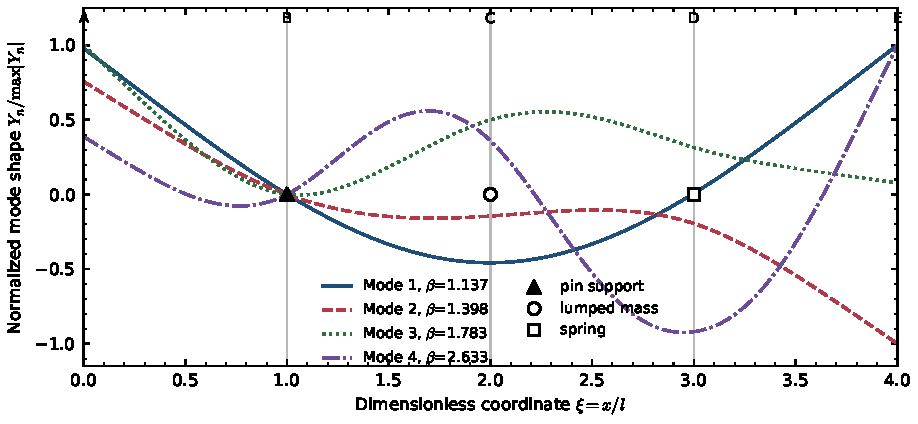
\includegraphics[width=\linewidth]{q3_mode_shapes.pdf}
    \caption{解析振型}
    \label{fig:analytical_modes}
  \end{subfigure}
  \hfill
  \begin{subfigure}{0.49\linewidth}
    \centering
    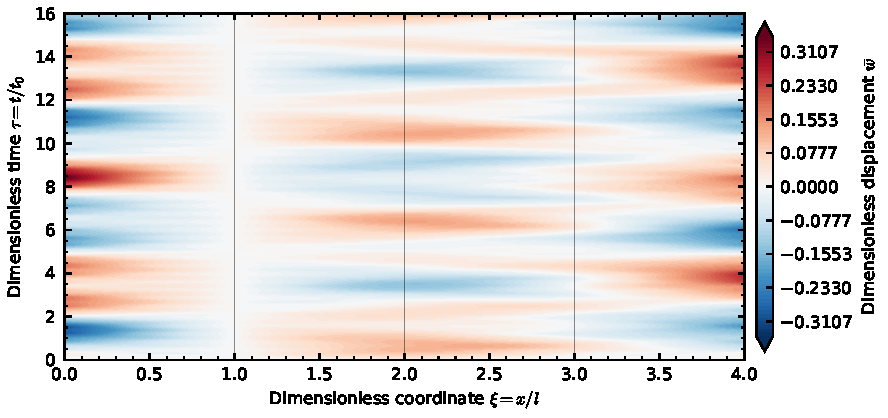
\includegraphics[width=\linewidth]{q3_spacetime_response.pdf}
    \caption{解析时空响应}
    \label{fig:analytical_spacetime}
  \end{subfigure}
  \caption{解析解振型与动力响应可视化}
  \label{fig:analytical_modes_response}
\end{figure}

\subsection{固有频率对比}

\cref{tab:freq_compare} 给出了前 $12$ 阶固有频率的解析解与有限元结果。可以看出，前 $11$ 阶频率误差均较小，第 $12$ 阶误差增大，说明在当前 $80$ 单元离散下，高阶模态已经开始受到空间离散误差影响。

\begin{table}[H]
\centering
\caption{解析解与有限元法固有频率对比}
\label{tab:freq_compare}
\small
\begin{tabular}{ccccc}
\toprule
阶数 & $\beta_n$ & 解析 $\bar\omega_n$ & FEM $\bar\omega_n$ & 相对误差/\%\\
\midrule
1 & 1.13706253 & 1.29291120 & 1.29291121 & $6.561\times10^{-7}$\\
2 & 1.39788505 & 1.95408261 & 1.95408264 & $1.614\times10^{-6}$\\
3 & 1.78311026 & 3.17948221 & 3.17948233 & $3.652\times10^{-6}$\\
4 & 2.63348065 & 6.93522035 & 6.93522170 & $1.953\times10^{-5}$\\
5 & 3.49807330 & 12.23651680 & 12.23652472 & $6.477\times10^{-5}$\\
6 & 4.12088500 & 16.98169320 & 16.98171295 & $1.163\times10^{-4}$\\
7 & 4.63075532 & 21.44389486 & 21.44393578 & $1.908\times10^{-4}$\\
8 & 5.49538421 & 30.19924764 & 30.19935982 & $3.715\times10^{-4}$\\
9 & 6.62342308 & 43.86973326 & 43.87010941 & $8.574\times10^{-4}$\\
10 & 7.22338705 & 52.17732044 & 52.17760933 & $5.537\times10^{-4}$\\
11 & 7.75075013 & 60.07412758 & 60.07546580 & $2.228\times10^{-3}$\\
12 & 8.58187870 & 73.64864210 & 73.67590498 & $3.702\times10^{-2}$\\
\bottomrule
\end{tabular}
\end{table}

\begin{figure}[H]
  \centering
  \begin{subfigure}{0.48\linewidth}
    \centering
    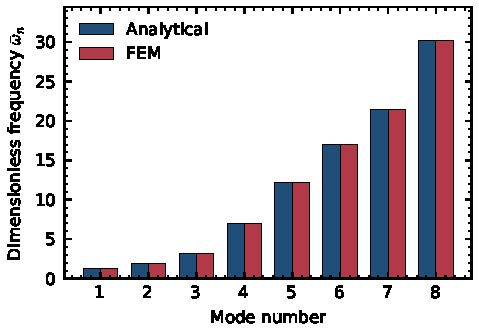
\includegraphics[width=\linewidth]{comparison_frequency_spectrum.pdf}
    \caption{前 8 阶频率对比}
    \label{fig:freq_bar}
  \end{subfigure}
  \hfill
  \begin{subfigure}{0.48\linewidth}
    \centering
    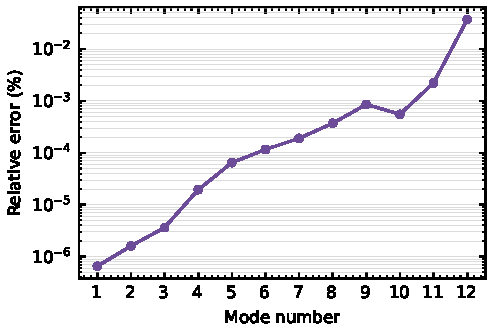
\includegraphics[width=\linewidth]{comparison_frequency_error.pdf}
    \caption{前 12 阶频率误差}
    \label{fig:freq_error}
  \end{subfigure}
  \caption{解析解与有限元法固有频率对比}
  \label{fig:freq_compare}
\end{figure}

\subsection{振型对比}

\cref{fig:mode_compare} 给出了前四阶振型叠合图。由于振型符号本身具有任意性，图中已按内积为正的原则对解析振型和有限元振型进行符号对齐。可以看到，两种方法得到的前四阶振型几乎完全重合。进一步计算节点振型差值，前四阶振型节点 $L_2$ 相对误差分别为 $2.455\times10^{-9}$、$1.727\times10^{-9}$、$2.404\times10^{-8}$ 和 $5.903\times10^{-8}$。

\begin{figure}[H]
  \centering
  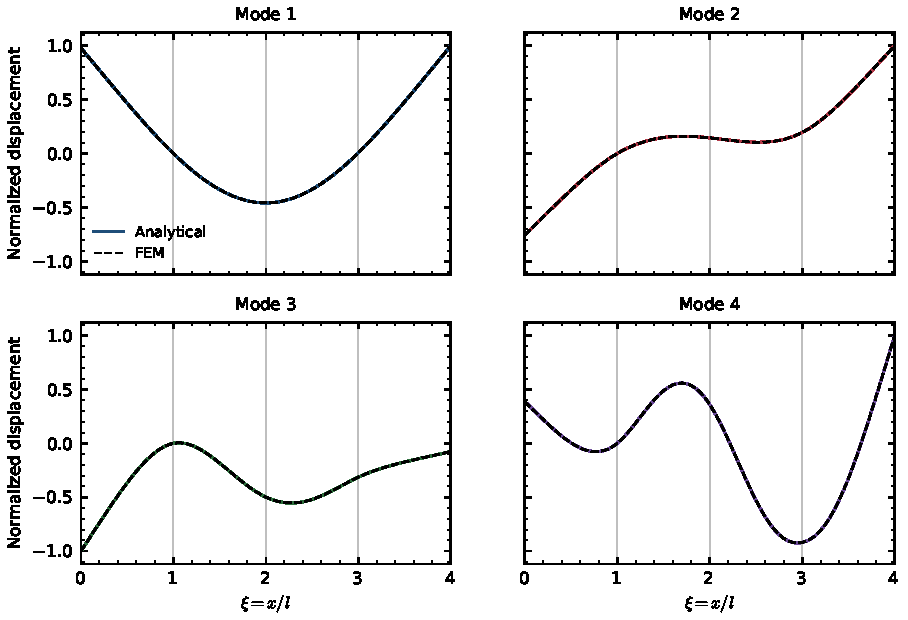
\includegraphics[width=0.92\linewidth]{comparison_mode_overlay.pdf}
  \caption{前四阶振型叠合对比}
  \label{fig:mode_compare}
\end{figure}

\begin{figure}[H]
  \centering
  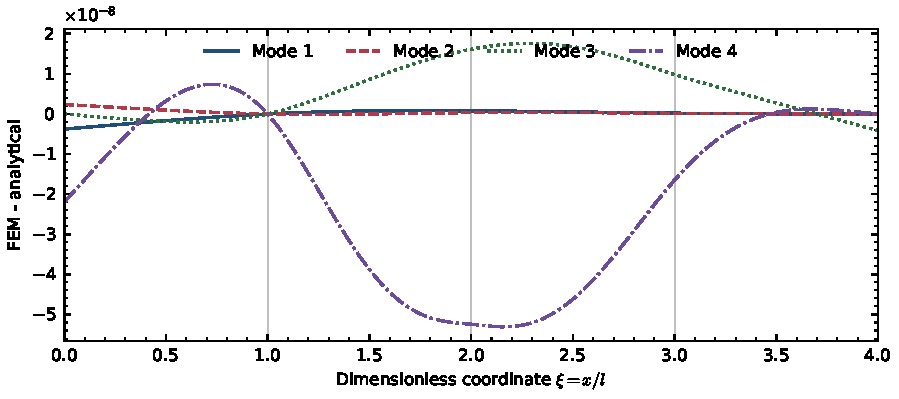
\includegraphics[width=0.92\linewidth]{comparison_mode_difference.pdf}
  \caption{前四阶振型差值曲线}
  \label{fig:mode_difference}
\end{figure}

\subsection{动力响应对比}

在初始位移为零、$C$ 点集中质量具有初速度 $v_0$ 的条件下，采用前 $24$ 阶模态叠加计算动力响应。\cref{fig:c_response} 给出了 $C$ 点位移与速度响应对比。位移响应中解析解与有限元法曲线基本重合；速度响应对高频模态更敏感，因此相对更容易体现有限元离散和模态截断带来的差异。

\begin{figure}[H]
  \centering
  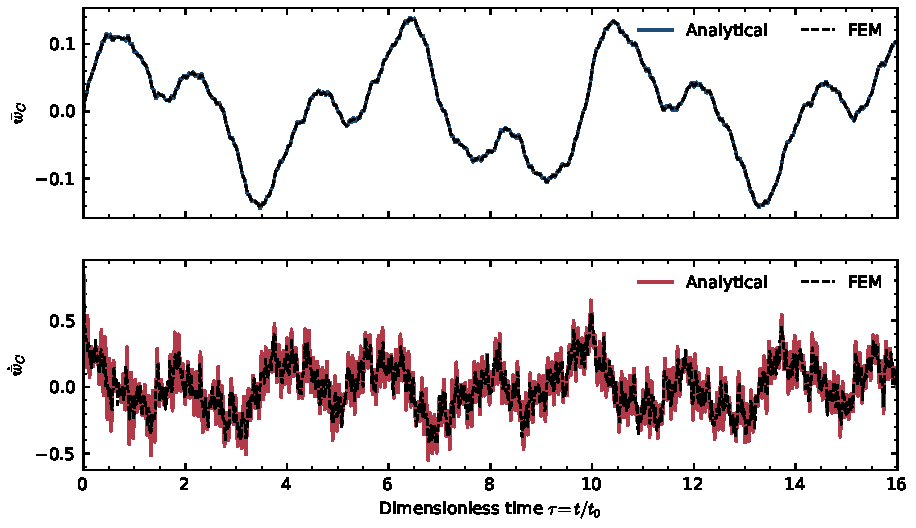
\includegraphics[width=0.92\linewidth]{comparison_c_response.pdf}
  \caption{$C$ 点位移与速度响应对比}
  \label{fig:c_response}
\end{figure}

\begin{figure}[H]
  \centering
  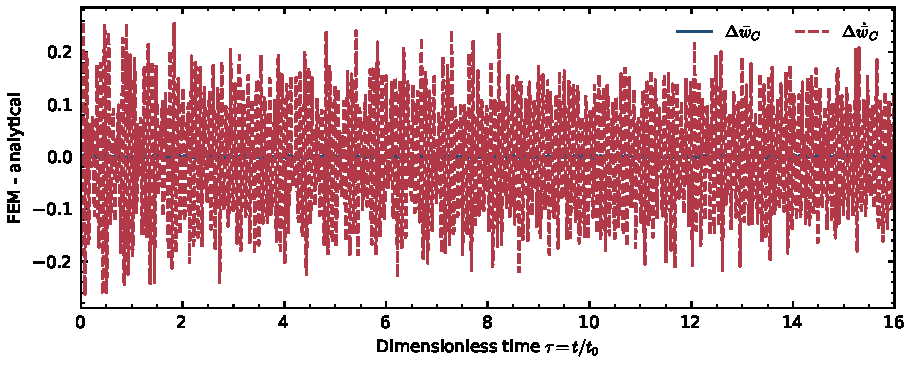
\includegraphics[width=0.92\linewidth]{comparison_c_response_error.pdf}
  \caption{$C$ 点响应差值}
  \label{fig:c_response_error}
\end{figure}

从全梁时空响应差值云图\cref{fig:field_difference} 可以看出，整体位移误差较小。计算得到 $C$ 点位移 RMS 误差为 $1.270\times10^{-3}$，$C$ 点速度 RMS 误差为 $1.008\times10^{-1}$，全梁时空位移 RMS 误差为 $3.086\times10^{-3}$，最大绝对误差为 $1.529\times10^{-2}$。该结果说明有限元模型能够较准确地捕捉结构的主导动力响应。

\begin{figure}[H]
  \centering
  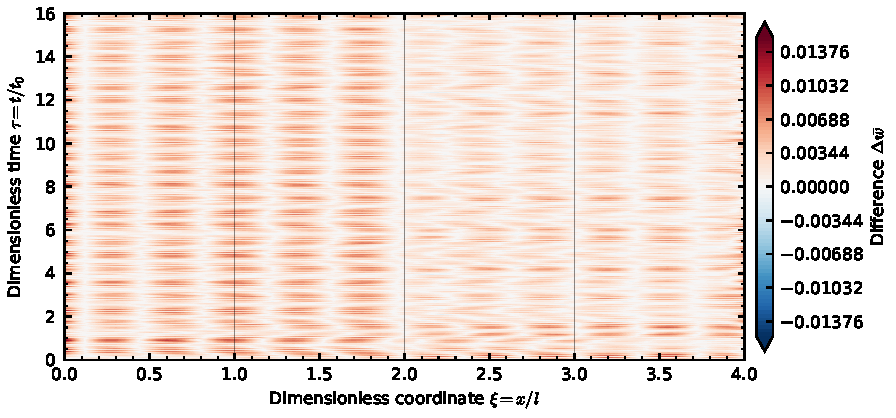
\includegraphics[width=0.92\linewidth]{comparison_spacetime_difference.pdf}
  \caption{全梁时空响应差值云图}
  \label{fig:field_difference}
\end{figure}

\section{结论}

本文针对一根含内点外部铰支、集中质量和局部竖向弹簧的 Euler--Bernoulli 梁，推导了横向自由振动解析解，并建立了有限元模型进行验证。主要结论如下：

\begin{enumerate}[label=(\arabic*)]
  \item 基于传递矩阵法可有效处理集中质量和弹簧支承引起的状态跳跃，所得特征方程能够统一描述该类分段连续梁结构的固有振动问题。
  \item 通过 Hermite 梁单元建立的有限元模型能够自然引入集中质量、局部弹簧和铰支约束，形成标准广义特征值问题。
  \item 在所取无量纲参数下，有限元前若干阶固有频率与解析解高度一致，前四阶振型与解析振型几乎完全重合，验证了理论推导和数值实现的正确性。
  \item 动力响应对比表明，位移响应吻合较好，速度响应对高阶模态更敏感。误差主要来源于有限元空间离散和模态截断，增加单元数及参与模态数可进一步提高响应精度。
\end{enumerate}

\begin{thebibliography}{9}
\bibitem{timoshenko}
Timoshenko S, Young D H, Weaver W.
Vibration Problems in Engineering.
New York: Wiley, 1974.

\bibitem{meirovitch}
Meirovitch L.
Analytical Methods in Vibrations.
New York: Macmillan, 1967.

\bibitem{clough}
Clough R W, Penzien J.
Dynamics of Structures.
Berkeley: Computers \& Structures, Inc., 2003.

\bibitem{cook}
Cook R D, Malkus D S, Plesha M E, Witt R J.
Concepts and Applications of Finite Element Analysis.
New York: Wiley, 2002.

\bibitem{rao}
Rao S S.
Mechanical Vibrations.
Upper Saddle River: Pearson, 2011.
\end{thebibliography}

\end{document}
